\documentclass[12pt]{extarticle}
\usepackage{titling}
\usepackage{lipsum}  
\usepackage[utf8]{inputenc}
\usepackage{polski}
\usepackage{geometry}
\usepackage{xcolor}
\geometry{
    a4paper,
    total={170mm,257mm},
    left=20mm,
    top=20mm,
}
\usepackage{graphicx}
\usepackage{wrapfig}
\usepackage{float}
\usepackage{amsmath}
\usepackage{multirow}

\pagenumbering{gobble}
\graphicspath{{./wykresy/}}

\pretitle{\begin{center}\Huge\bfseries}
\posttitle{\par\end{center}\vskip 0.4em}
\preauthor{\begin{center}\Large}
\postauthor{\end{center}}
\predate{\par\large\centering}
\postdate{\par} 

\begin{document}
\title{
    Aproksymacja profilu wysokościowego \\
    \large Metody Numeryczne - Projekt 3
}

\author{Krystian Jandy, 184589 - Grupa 2}
\date{Maj 2022}

\maketitle

\section*{Wprowadzenie}
 Celem projektu z przedmiotu Metod Numerycznych jest implementacja metody wykorzystującej wielomian interpolacyjny Lagrange oraz metodę wykorzystującą funkcje sklejane trzeciego stopnia, które to metody są potrzebne do utworzenia profilu wysokościowego na podstawie wybranych węzłów interpolacyjnych.\\
 Do realizacji projektu został użyty język Python, natomiast do wizualizacji utworzonego profilu wysokościowego wykorzystano biblioteke matplotlib.
\section*{Wybrane trasy}
\begin{itemize}
    \item \textbf{Wielki Kanion w Kolorado}\\
    Teren z wyraźną różnicą wysokości (występują wzniesienia oraz spadki)
    \begin{figure}[H]
        \centering
        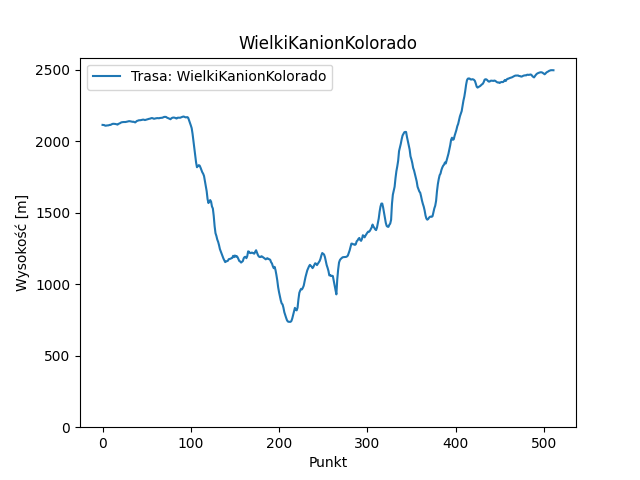
\includegraphics[scale=0.8]{WielkiKanionKolorado.png}
        \caption{Wykres przedstawiający profil wysokościowy Wielkiego Kanionu w Kolorado}
    \end{figure}
    \item \textbf{Mount Everest}\\
    Teren górzysty, występuje jedno znaczne wzniesienie
    \begin{figure}[H]
        \centering
        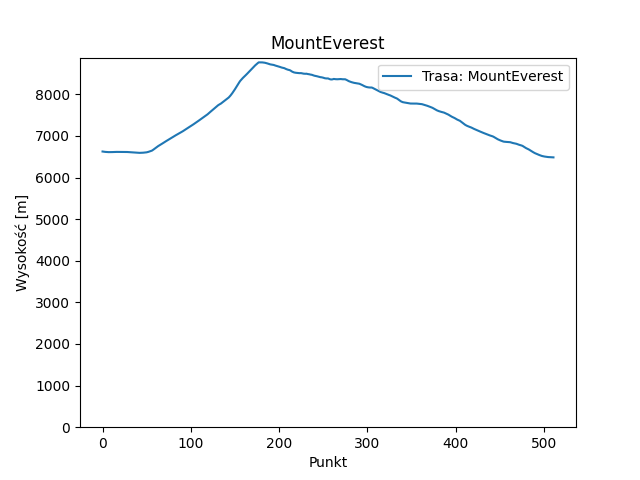
\includegraphics[scale=0.8]{MountEverest.png}
        \caption{Wykres przedstawiający profil wysokościowy szczytu Mount Everest}
    \end{figure}
    \item \textbf{Chełm}\\
    Trasa bez znaczących różnic wysokościowego (prawie płaska)
    \begin{figure}[H]
        \centering
        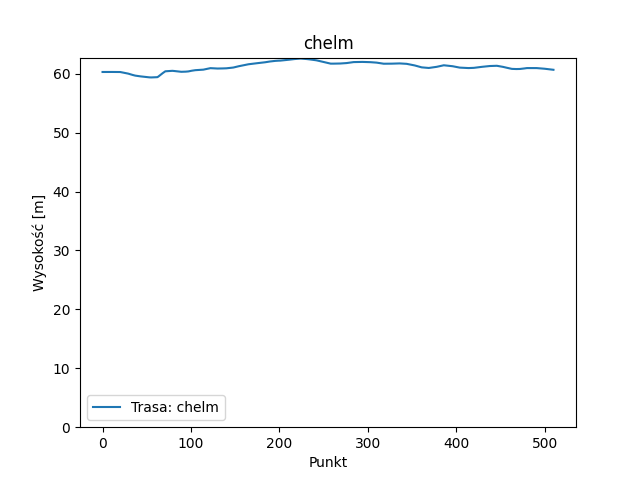
\includegraphics[scale=0.8]{chelm.png}
        \caption{Wykres przedstawiający profil wysokościowy na Chełmie}
    \end{figure}
    \item \textbf{Spacerniak w Gdańsku}\\
    Zróżnicowana trasa, gdzie występują na przemian wzniesienia oraz spadki.
    \begin{figure}[H]
        \centering
        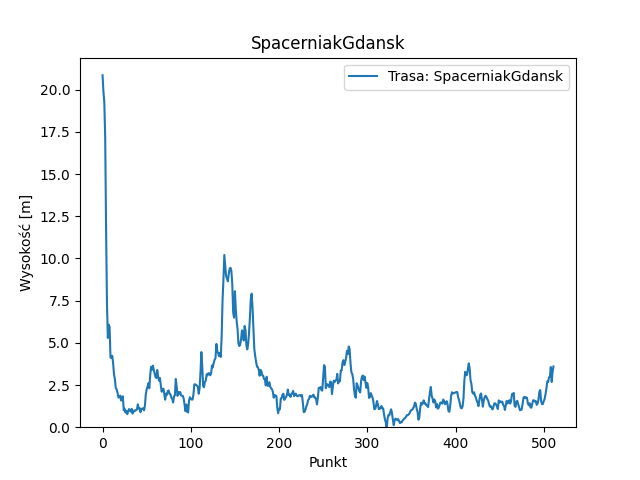
\includegraphics[scale=0.8]{SpacerniakGdansk.png}
        \caption{Wykres przedstawiający profil wysokościowy na spacerniaku w Gdańsku}
    \end{figure}
\end{itemize}

\section*{Liczba punktów węzłowych}
W celu zbadania powyższych metod przeprowadzono analize na \textbf{3, 6, 11, 35, 52, 103} punktach węzłowych, będących wyróżnionymi punktami ze zbioru danych wejściowych. 

\section*{Interpolacja Lagrange'a}
Interpolacja Lagrange'a to łatwa w implementacji metoda bazująca na wyznaczeniu wielomianu n-tego stopnia określonego przez n+1 punktów. Baza Lagrange do interpolacji składa się z funkcji określonych wzorem:
\begin{equation}
    \phi_{i}(x) = \prod_{j=1, j \neq i}^{n+1}\frac{(x - x_{j})}{(x_{i} - x_{j})}, dla\;i = 1,2 \ldots n+1
\end{equation} 
W interpolacji Lagrange'a nie trzeba konstruować i rozwiązywać układu równań liniowych, co jest jednym z etapów interpolacji funkcjami sklejanymi. Jednakże ta metoda jest podatna na \textbf{efekt Rungego} co charakterysuje się tym, że na krawędziach pojawiają się oscylację.
\subsection*{Wpływ liczby węzłów na wyniki}
Liczba węzłów znacząco oddziałuję na uzyskany wynik.    Można zauważyć, że wraz ze wzrostem liczby węzłów funkcja jest dobrze interpolowana w środku przedziału, jednakze na krawędziach pojawiają się oscylacje.
\newpage
\textbf{Przykład wpływu liczby węzłów na wyniki zaprezentowany na trasie Mount Everest:}
\begin{figure}[H]
    \centering
    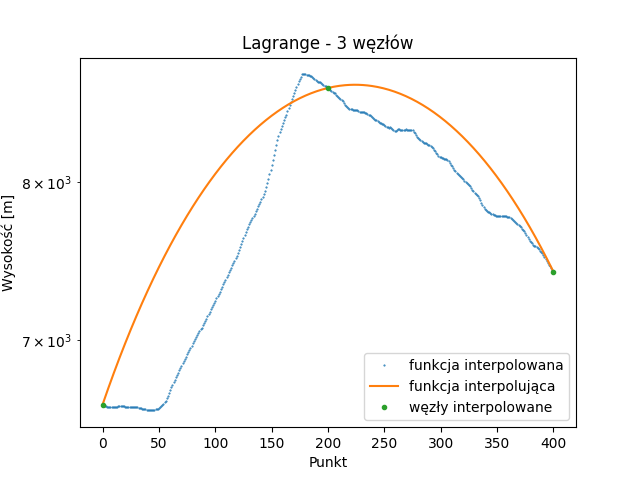
\includegraphics[scale=0.8]{interpolation_MountEverest_Lagrange_3.png}
    \caption{Mount Everest - Interpolacja Lagrange'a dla 3 węzłów}
\end{figure}
\begin{figure}[H]
    \centering
    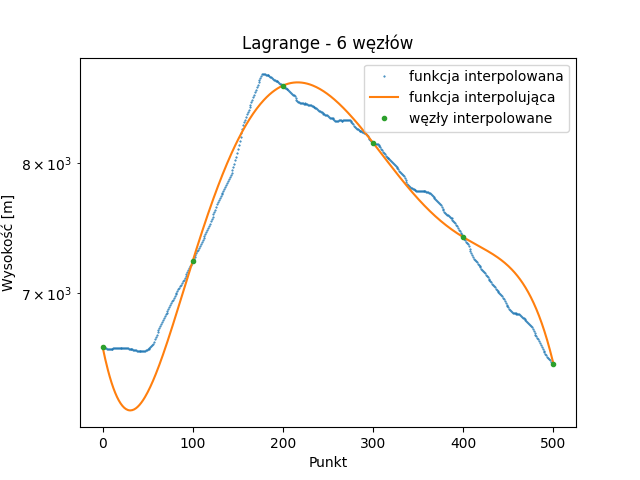
\includegraphics[scale=0.8]{interpolation_MountEverest_Lagrange_6.png}
    \caption{Mount Everest - Interpolacja Lagrange'a dla 6 węzłów}
\end{figure}
\begin{figure}[H]
    \centering
    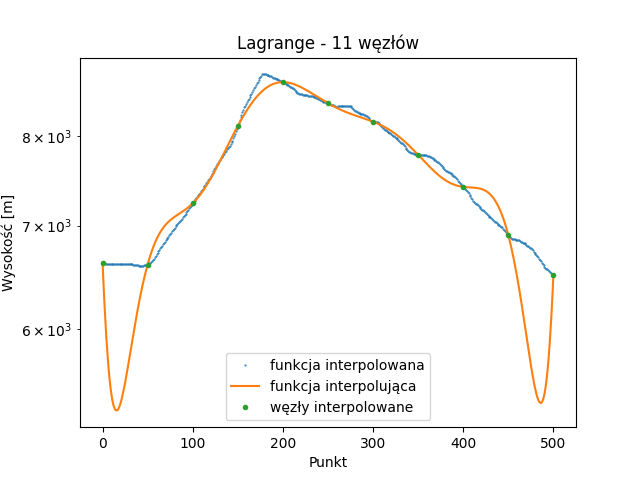
\includegraphics[scale=0.8]{interpolation_MountEverest_Lagrange_11.png}
    \caption{Mount Everest - Interpolacja Lagrange'a dla 11 węzłów}
\end{figure}
\begin{figure}[H]
    \centering
    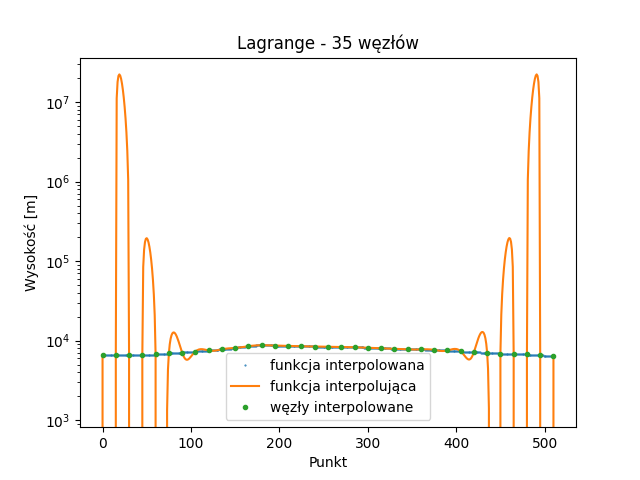
\includegraphics[scale=0.8]{interpolation_MountEverest_Lagrange_35.png}
    \caption{Mount Everest - Interpolacja Lagrange'a dla 35 węzłów}
\end{figure}
\begin{figure}[H]
    \centering
    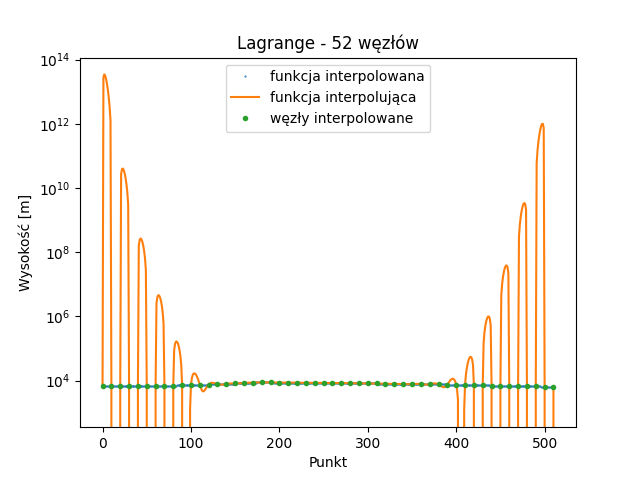
\includegraphics[scale=0.8]{interpolation_MountEverest_Lagrange_52.png}
    \caption{Mount Everest - Interpolacja Lagrange'a dla 52 węzłów}
\end{figure}
\begin{figure}[H]
    \centering
    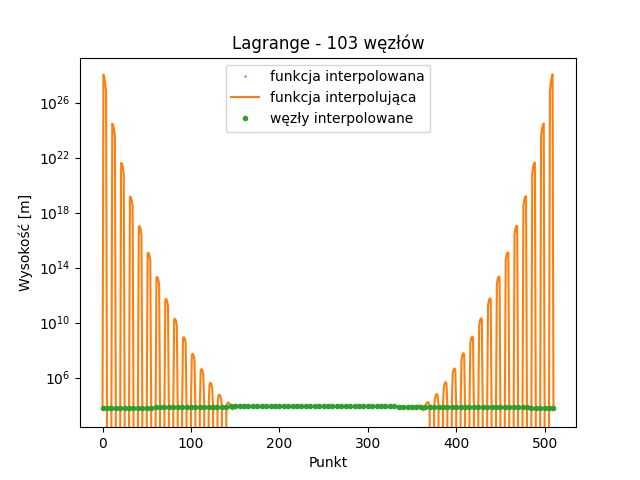
\includegraphics[scale=0.8]{interpolation_MountEverest_Lagrange_103.png}
    \caption{Mount Everest - Interpolacja Lagrange'a dla 103 węzłów}
\end{figure}
Z otrzymanych wyników można wywnioskować, że funkcja jest dobrze interpolowana w środku, natomiast wraz z wzrostem punktów interpolujących znacząco daje się zauważyć efekt Rungego.
\subsubsection*{Wpływ rozmieszczenia punktów węzłowych na wyniki}
W celu zaprezentowania wpływu rozmieszczenia punktów węzłowych na wyniki posłużono się trasą przedstawiającą spacerniak w Gdańsku.
\begin{figure}[H]
    \centering
    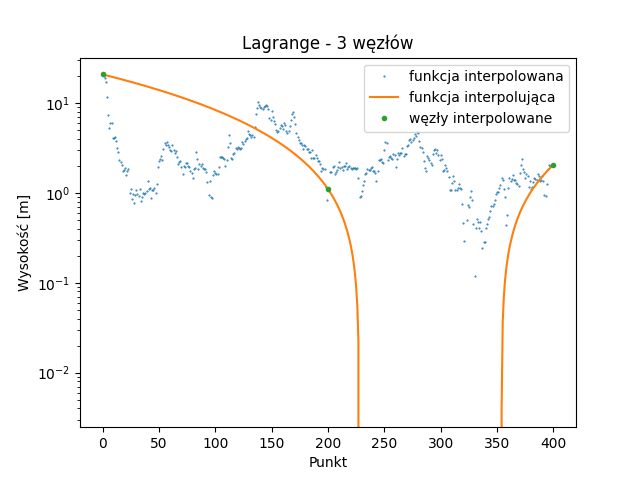
\includegraphics[scale=0.8]{interpolation_SpacerniakGdansk_Lagrange_3.png}
    \caption{Spacerniak w Gdańsku - Interpolacja Lagrange'a dla 3 węzłów}
\end{figure}
\begin{figure}[H]
    \centering
    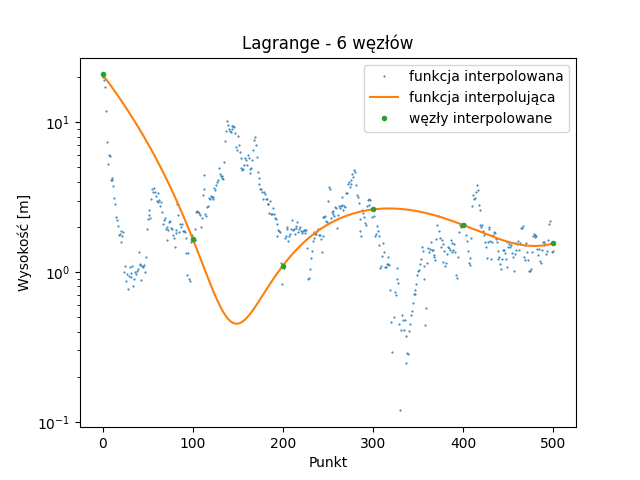
\includegraphics[scale=0.8]{interpolation_SpacerniakGdansk_Lagrange_6.png}
    \caption{Spacerniak w Gdańsku - Interpolacja Lagrange'a dla 6 węzłów}
\end{figure}
\begin{figure}[H]
    \centering
    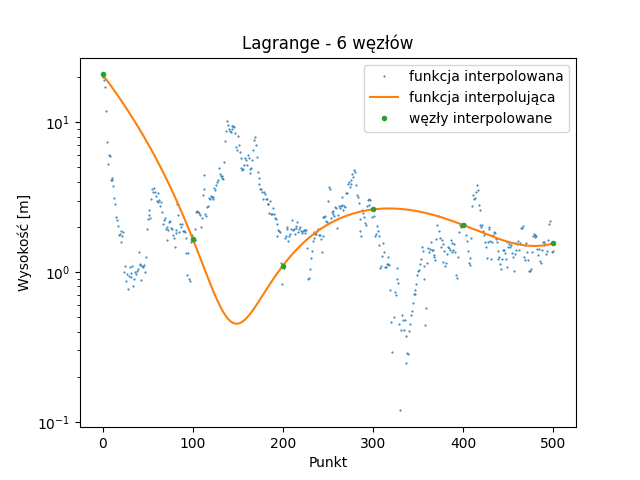
\includegraphics[scale=0.8]{interpolation_SpacerniakGdansk_Lagrange_6.png}
    \caption{Spacerniak w Gdańsku - Interpolacja Lagrange'a dla 6 węzłów}
\end{figure}
\begin{figure}[H]
    \centering
    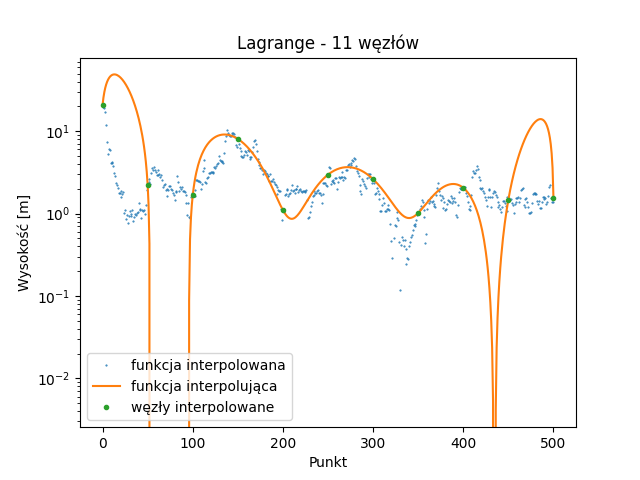
\includegraphics[scale=0.8]{interpolation_SpacerniakGdansk_Lagrange_11.png}
    \caption{Spacerniak w Gdańsku - Interpolacja Lagrange'a dla 11 węzłów}
\end{figure}
\begin{figure}[H]
    \centering
    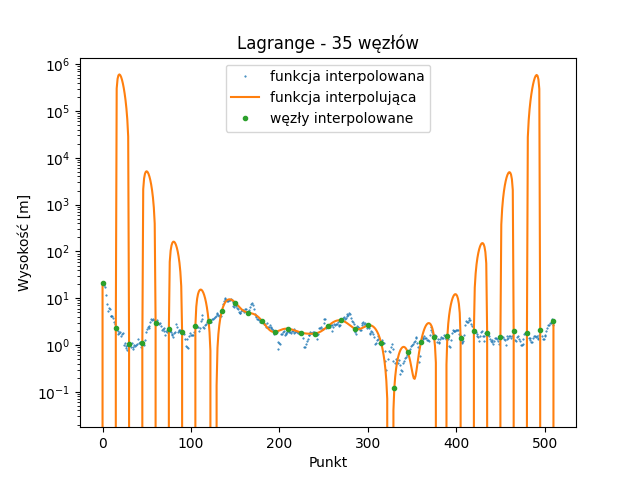
\includegraphics[scale=0.8]{interpolation_SpacerniakGdansk_Lagrange_35.png}
    \caption{Spacerniak w Gdańsku - Interpolacja Lagrange'a dla 35 węzłów}
\end{figure}
\begin{figure}[H]
    \centering
    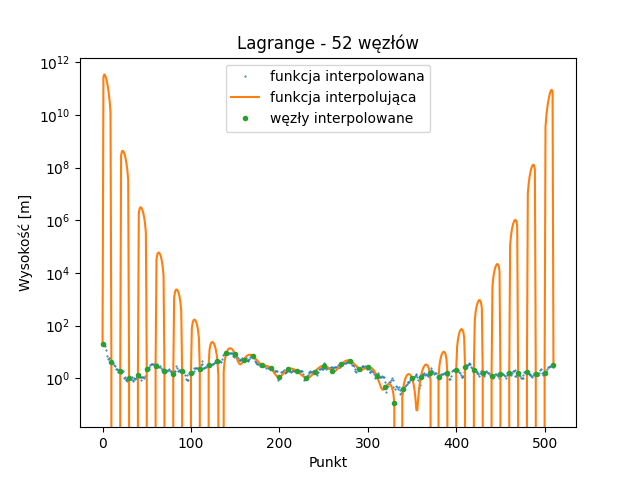
\includegraphics[scale=0.8]{interpolation_SpacerniakGdansk_Lagrange_52.png}
    \caption{Spacerniak w Gdańsku - Interpolacja Lagrange'a dla 52 węzłów}
\end{figure}
\begin{figure}[H]
    \centering
    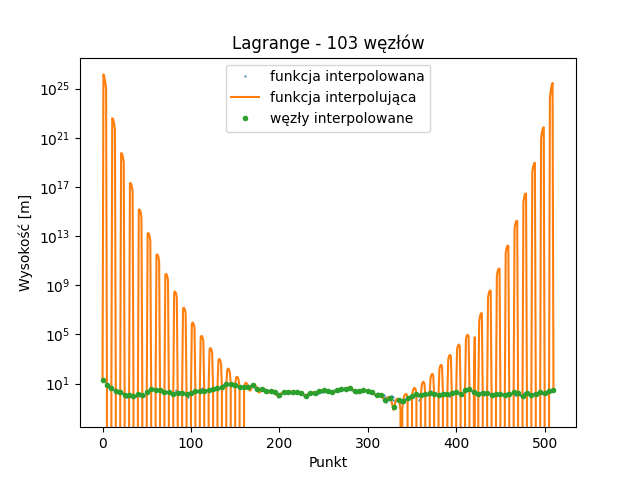
\includegraphics[scale=0.8]{interpolation_SpacerniakGdansk_Lagrange_103.png}
    \caption{Spacerniak w Gdańsku - Interpolacja Lagrange'a dla 103 węzłów}
\end{figure}
Z otrzymanych wyników można wyciągnąć wniosek że rozmieszczenie punktów ma znaczący wpływ na wynik, jak widać przy rzadkim rozmieszczeniu punktów pomijane są pewne zmiany wysokości co można zauważyć przy 6 węzłach dla metody Lagrange, gdzie pomijany jest ewidentny wzrost wysokości.
\subsubsection*{Wpływ charakteru trasy na wyniki}
Na powyższych wykresach można zauważyć, że charakter terenu ma znaczący wpływ na wyniki, przy terenie gdzie nie ma częstej zmiany wysokości aproksymacja jest dokładniejsza (Mount Everest), niż w terenie gdzie na przemian występują wzniesienia i strome spadki (Spacerniak w Gdańsku), przez tak częste zmiany wysokości są one pomijane.

\section*{Interpolacja funkcjami sklejanymi (splajnami)}
Ze względu na to, że interpolacja globalna (Lagrange'a) jest ryzykowna i podatna na wystąpienie efektu Rungego stosuje się interpolacje lokalną (występującą pomiędzy poszczególnymi węzłami) z użyciem wielomianu 3 stopnia. W tej metodzie stosuje się n przedziałów dla n+1 punktów, jednakże ta metoda jest bardziej złożona obliczeniowo ponieważ musimy dla każdego podprzedziału utworzyć funkcję co wiąże się z utworzeniem układu równań, w celu wyznaczenia współczynników funkcji dla każdego z podprzedziału.
\subsection*{Wpływ liczby węzłów na wyniki}
Podobnie jak w metodzie Lagrange'a wraz ze wzrostem liczby węzłów otrzymana aproksymacja jest dużo dokładniejsza, dodatkowo w interpolacji funkcjami skeljanymi nie występuje efekt Rungego.
\newpage
\textbf{Przykład wpływu liczby węzłów na wyniki zaprezentowany na trasie Mount Everest:}
\begin{figure}[H]
    \centering
    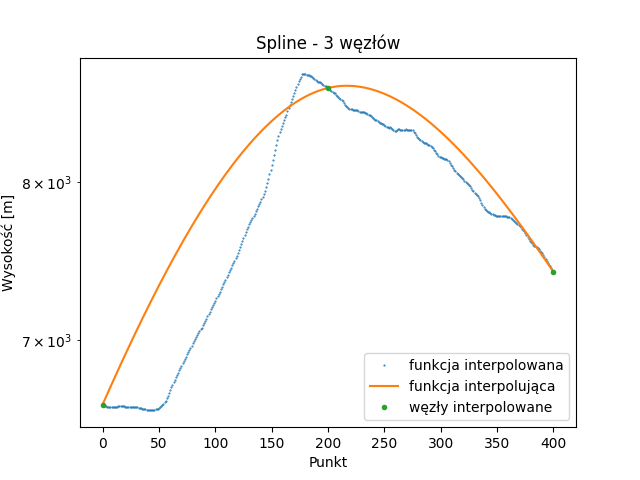
\includegraphics[scale=0.8]{interpolation_MountEverest_Spline_3.png}
    \caption{Mount Everest - Interpolacja funkcjami sklejanymi dla 3 węzłów}
\end{figure}
\begin{figure}[H]
    \centering
    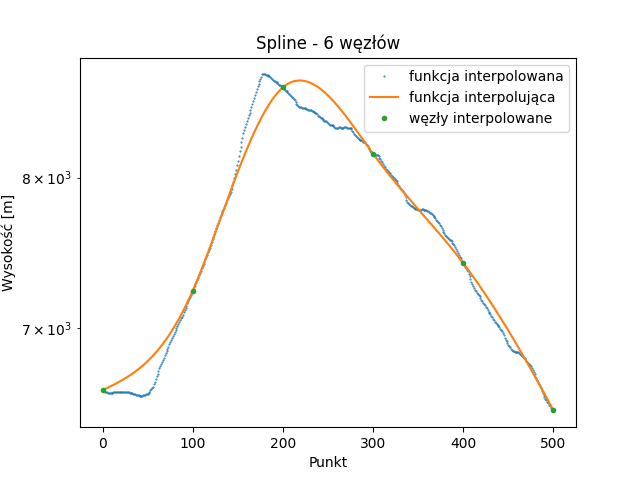
\includegraphics[scale=0.8]{interpolation_MountEverest_Spline_6.png}
    \caption{Mount Everest - Interpolacja funkcjami sklejanymi dla 6 węzłów}
\end{figure}
\begin{figure}[H]
    \centering
    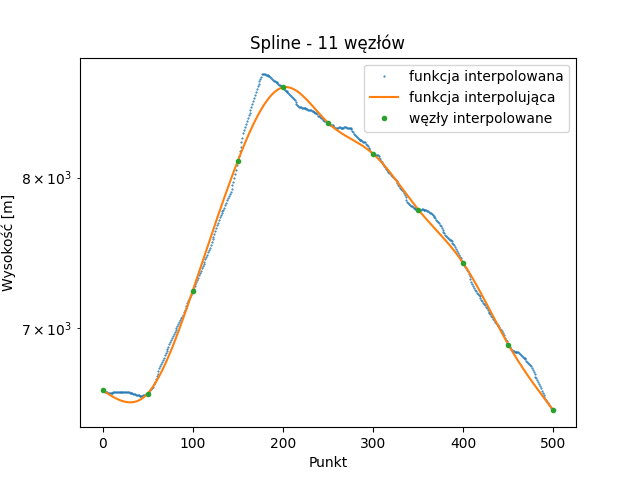
\includegraphics[scale=0.8]{interpolation_MountEverest_Spline_11.png}
    \caption{Mount Everest - Interpolacja funkcjami sklejanymi dla 11 węzłów}
\end{figure}
\begin{figure}[H]
    \centering
    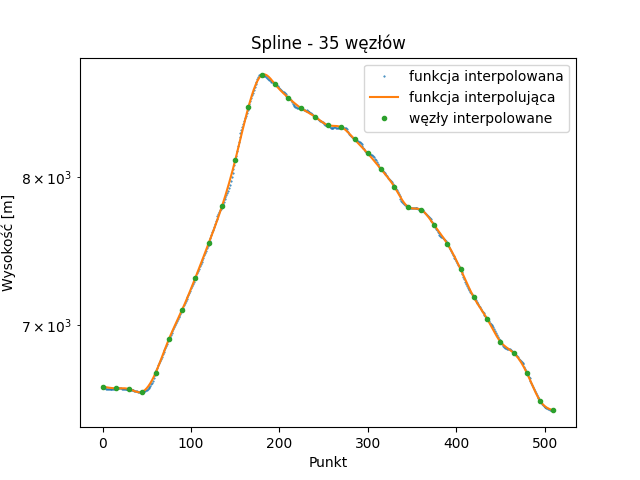
\includegraphics[scale=0.8]{interpolation_MountEverest_Spline_35.png}
    \caption{Mount Everest - Interpolacja funkcjami sklejanymi dla 35 węzłów}
\end{figure}
\begin{figure}[H]
    \centering
    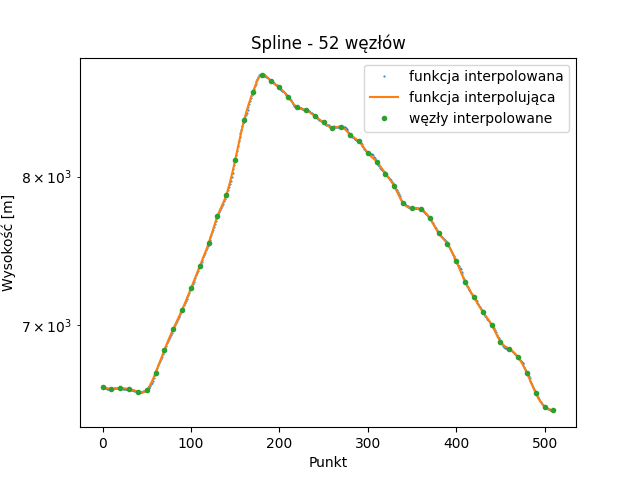
\includegraphics[scale=0.8]{interpolation_MountEverest_Spline_52.png}
    \caption{Mount Everest - Interpolacja funkcjami sklejanymi dla 52 węzłów}
\end{figure}
\begin{figure}[H]
    \centering
    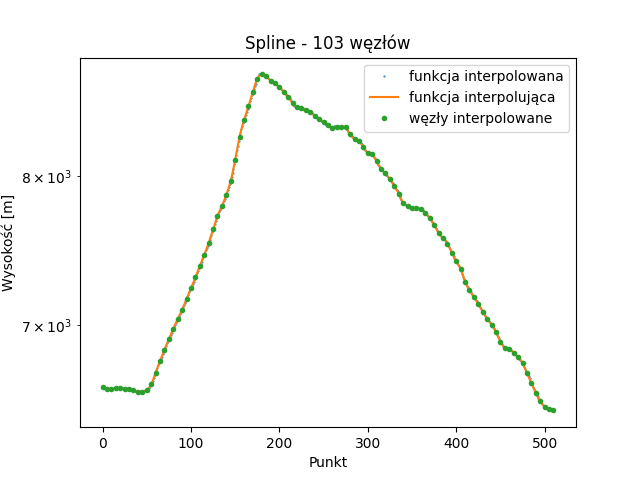
\includegraphics[scale=0.8]{interpolation_MountEverest_Spline_103.png}
    \caption{Mount Everest - Interpolacja funkcjami sklejanymi dla 103 węzłów}
\end{figure}
Jak można zauważyc wynik w przypadku interpolowania terenu Mount Everest jest już zadowalający przy inteprolowaniu z wykorzystaniem 35 węzłów.
\subsubsection*{Wpływ rozmieszczenia punktów węzłowych na wyniki}
Rozmieszczenie punktów węzłowych w metodzie  interpolacji funkcjami sklejanymi również jak to było w przypadku metodzie Lagrange'a ma istotny wpływ na otrzymany wynik, co można zauważyć na poniżej przedstawionym przykładzie.
\begin{figure}[H]
    \centering
    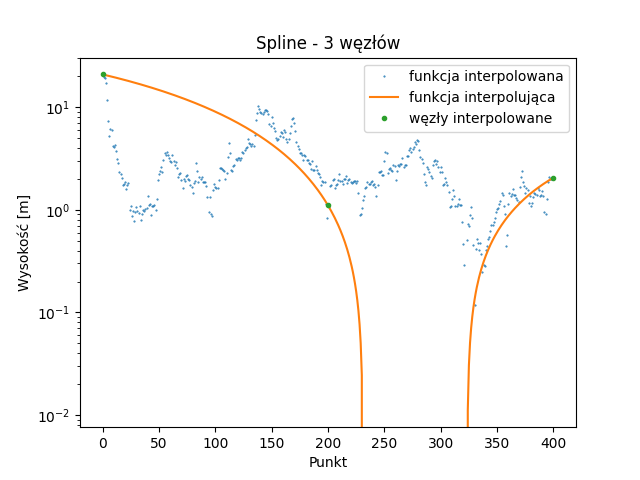
\includegraphics[scale=0.8]{interpolation_SpacerniakGdansk_Spline_3.png}
    \caption{Spacerniak w Gdańsku - Interpolacja funkcjami sklejanymi dla 3 węzłów}
\end{figure}
\begin{figure}[H]
    \centering
    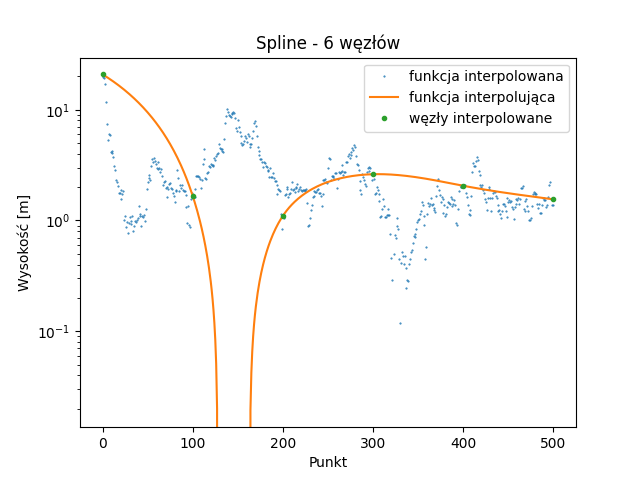
\includegraphics[scale=0.8]{interpolation_SpacerniakGdansk_Spline_6.png}
    \caption{Spacerniak w Gdańsku - Interpolacja funkcjami sklejanymi dla 6 węzłów}
\end{figure}
\begin{figure}[H]
    \centering
    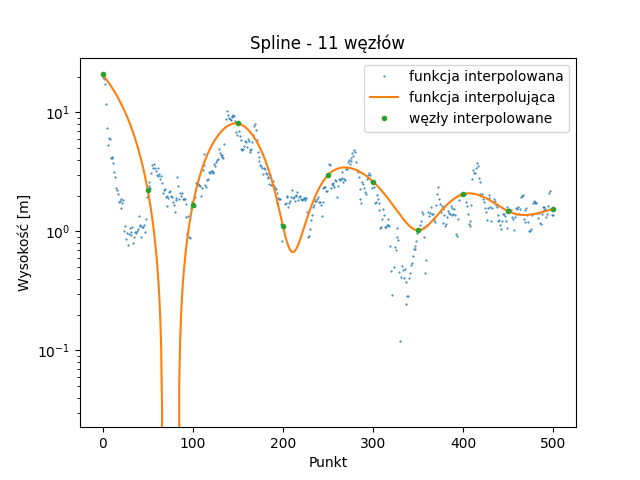
\includegraphics[scale=0.8]{interpolation_SpacerniakGdansk_Spline_11.png}
    \caption{Spacerniak w Gdańsku - Interpolacja funkcjami sklejanymi dla 11 węzłów}
\end{figure}
\begin{figure}[H]
    \centering
    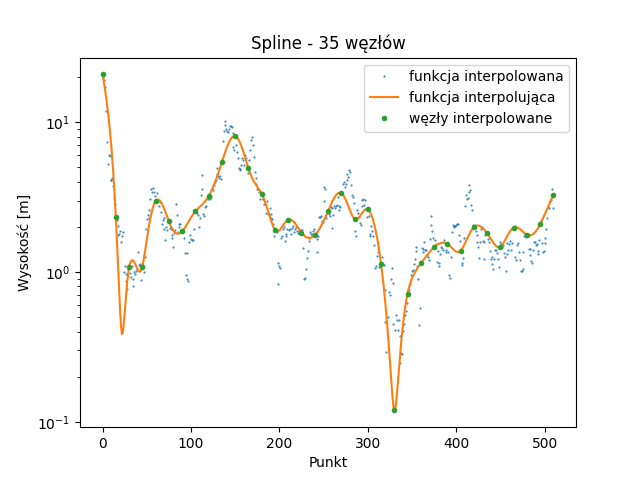
\includegraphics[scale=0.8]{interpolation_SpacerniakGdansk_Spline_35.png}
    \caption{Spacerniak w Gdańsku - Interpolacja funkcjami sklejanymi dla 35 węzłów}
\end{figure}
\begin{figure}[H]
    \centering
    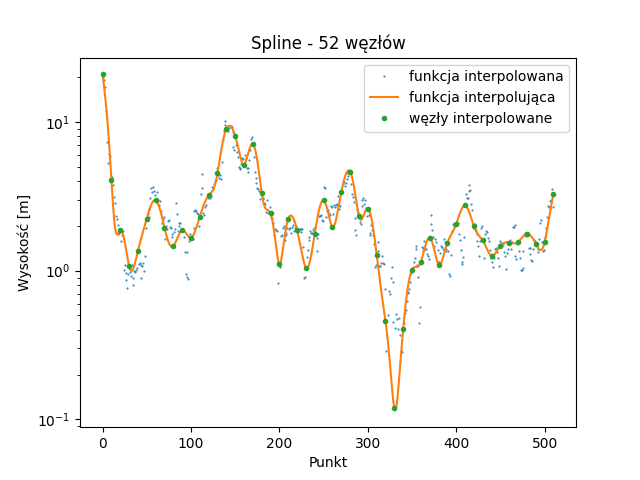
\includegraphics[scale=0.8]{interpolation_SpacerniakGdansk_Spline_52.png}
    \caption{Spacerniak w Gdańsku - Interpolacja funkcjami sklejanymi dla 52 węzłów}
\end{figure}
\begin{figure}[H]
    \centering
    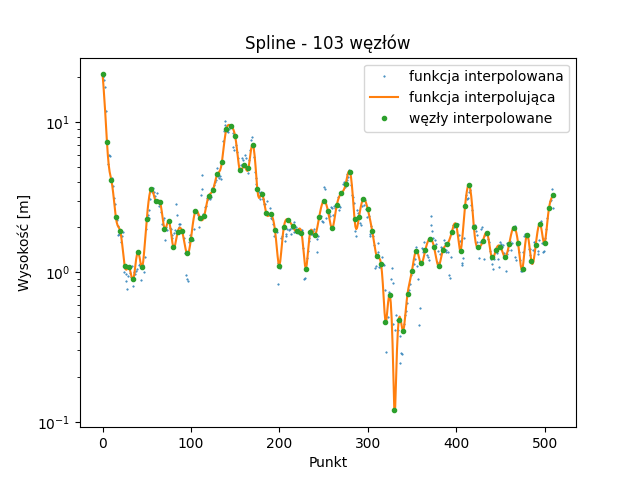
\includegraphics[scale=0.8]{interpolation_SpacerniakGdansk_Spline_103.png}
    \caption{Spacerniak w Gdańsku - Interpolacja funkcjami sklejanymi dla 103 węzłów}
\end{figure}
Przedstawione wykresy prezentują wpływ rozmieszczenia punktów na dokładność aproksymacji. Można zauważyć, że wraz ze wzrostem zagęszczenia punktów aproksymacja jest dokładniejsza.
\subsubsection*{Wpływ charakteru trasy na wyniki}
Podobnie jak to było w poprzedniej metodzie, charakter trasy ma wpływ na otrzymany wynik, ponieważ to czy trasa ma tendencje do licznej zmiany wysokości wiąże się z tym, że interpolacja bedzie mniej dokładna, niż w przypadku trasy gdzie ta wysokość oscyluje na podobnych wartościach, bądź występuje na całej trasie tendencja wzrostu lub spadku. Prezentuje to przykład powyżej, gdzie na spacerniaku w Gdańsku interpolacja dla 52 węzłów nie osiąga takiego rezultatu jak możemy zauważyć dla interpolowania terenu Mount Everest, bądź poniżej przedstawionego terenu Chełmu, w których to już interpolacja dla 35 węzłów daje zadowalający wynik.
\begin{figure}[H]
    \centering
    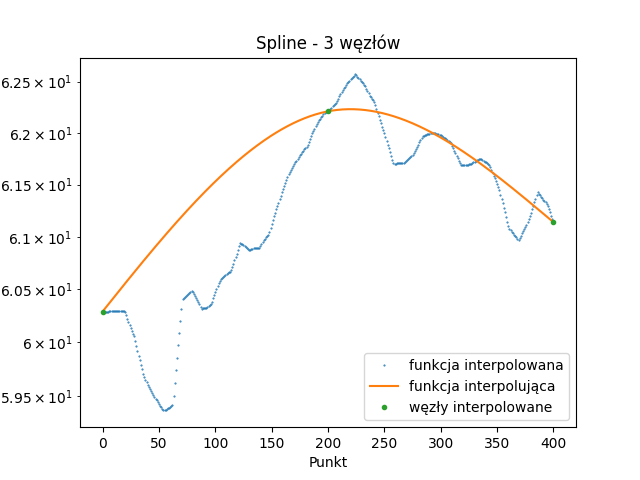
\includegraphics[scale=0.65]{interpolation_chelm_Spline_3.png}
    \caption{Chełm - Interpolacja funkcjami sklejanymi dla 3 węzłów}
\end{figure}
\begin{figure}[H]
    \centering
    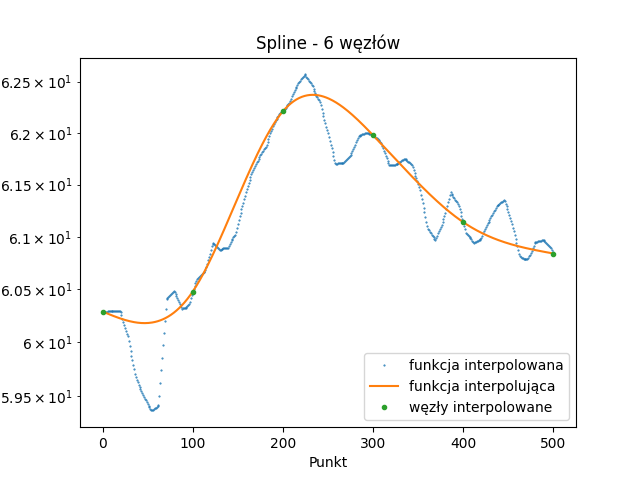
\includegraphics[scale=0.65]{interpolation_chelm_Spline_6.png}
    \caption{Chełm - Interpolacja funkcjami sklejanymi dla 6 węzłów}
\end{figure}
\begin{figure}[H]
    \centering
    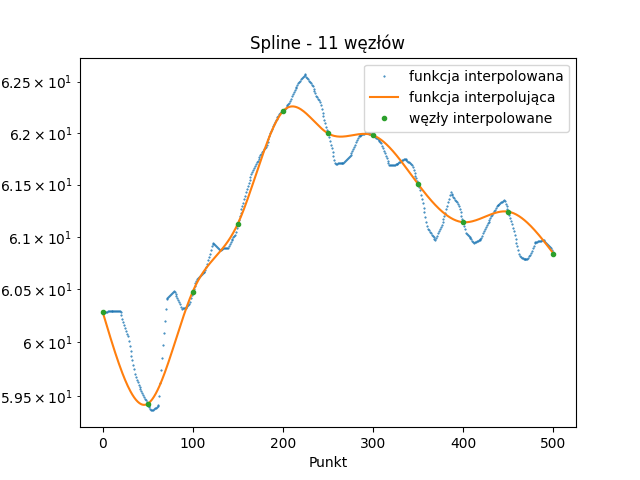
\includegraphics[scale=0.8]{interpolation_chelm_Spline_11.png}
    \caption{Chełm - Interpolacja funkcjami sklejanymi dla 11 węzłów}
\end{figure}
\begin{figure}[H]
    \centering
    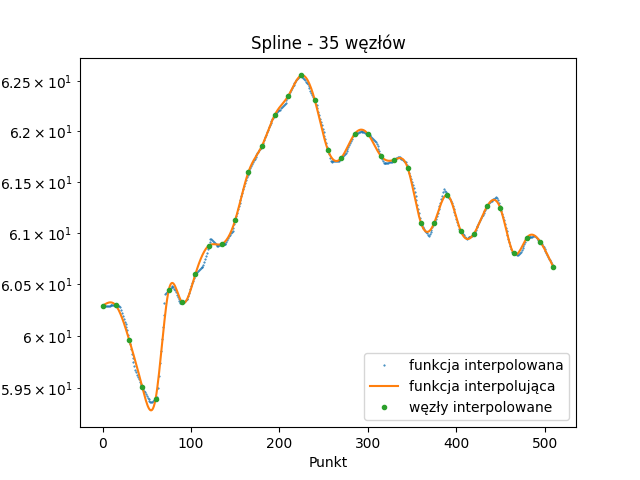
\includegraphics[scale=0.8]{interpolation_chelm_Spline_35.png}
    \caption{Chełm - Interpolacja funkcjami sklejanymi dla 35 węzłów}
\end{figure}
\begin{figure}[H]
    \centering
    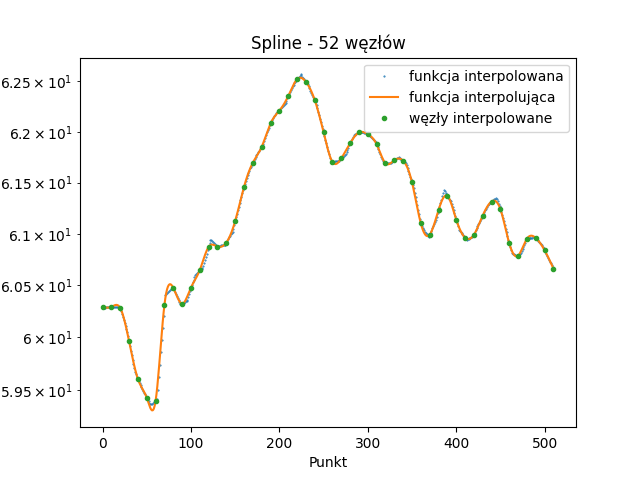
\includegraphics[scale=0.8]{interpolation_chelm_Spline_52.png}
    \caption{Chełm - Interpolacja funkcjami sklejanymi dla 52 węzłów}
\end{figure}
\begin{figure}[H]
    \centering
    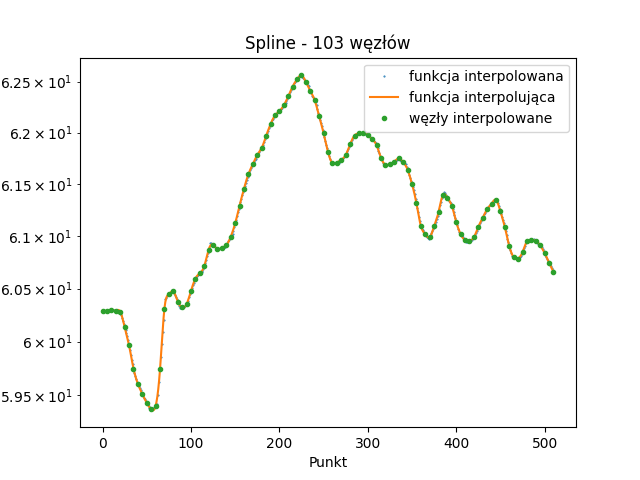
\includegraphics[scale=0.8]{interpolation_chelm_Spline_103.png}
    \caption{Chełm - Interpolacja funkcjami sklejanymi dla 103 węzłów}
\end{figure}
\newpage
\section*{Podsumowanie}
\textbf{Wpływ liczby punktów węzłowych na wyniki}\\
Liczba punktów węzłowych ma znaczący wpływ na wyniki, w obu metodach wraz ze wzrostem liczby punktów zwiększa się dokładność aproksymacji (jednakże w przypadku metody Lagrange'a pojawia się problem Rungego).
\\ \\
\textbf{Wpływ rozmieszczenia punktów węzłowych na wyniki}\\
Równomierne rozmieszczenie punktów węzłowych poprawia wynik.
\\ \\
\textbf{Wpływ charakteru trasy na wyniki}\\
Trasy, które charakteryzują się gwałtownymi zmianami tendencji wzrostu (wzniosy/spadki na przemian) potrzebują większej liczby punktów interpolowanych aby otrzymać dokładny wynik, natomiast trasy o stałej tendencji wzrostu/spadku, bądź trasy płaskie potrzebują mniej węzłów interpolujących w celu uzyskania zadowalającego wyniku.\\ 
\\
Interpolacja funkcjami skeljanymi jest metodą kosztowniejszą obliczeniowo, natomiast daje zadowalające wyniki aproksymacji punktów dyskretnych. Nie występuje tam efekt Rungego, który jest widoczny w metodach globalnych interpolacji. 
\end{document} 